\chapter*{Введение}

В настоящее время как в нашей стране, так и за рубежом всё большее внимание уделяется созданию различных типов беспилотных летательных аппаратов (БПЛА)~\cite{UAVBook}. 


Различными компаниями разработаны и практически реализованы многочисленные проекты БПЛА, предназначенные для решения различного рода задач как для гражданских, так и для военных задач. На Рис.\ref{fig:UAVs} представлены некоторые из существующих БПЛА с указанием их предназначения.


\begin{figure}[H]
        \begin{subfigure}[b]{0.47\textwidth}
                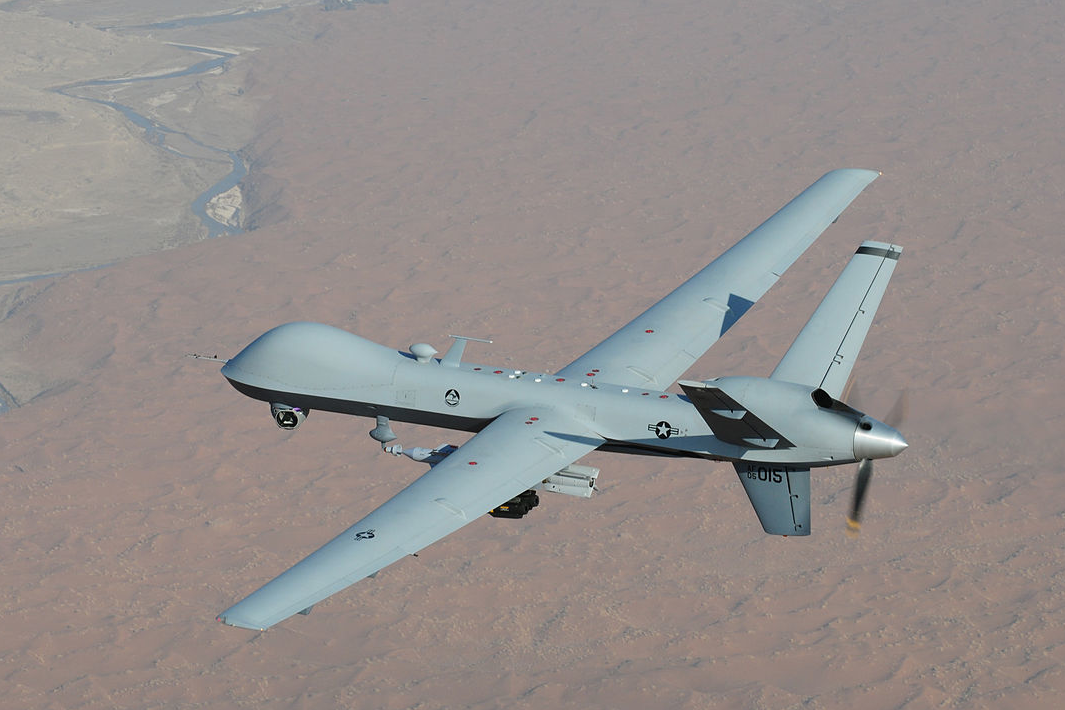
\includegraphics[width=\linewidth]{UAV_Reaper}
                \caption{MQ-9 Reaper, разведывательно-ударный} % http://ru.wikipedia.org/wiki/MQ-9_Reaper , U.S. Air Force Photo / Lt. Col. Leslie Pratt - USAF Photographic Archives http://www.afrc.af.mil/shared/media/photodb/photos/090127-F-7383P-002.JPG
                \label{fig:UAV_Reaper}
        \end{subfigure}%
        \hspace{\fill}
        \begin{subfigure}[b]{0.47\textwidth}
                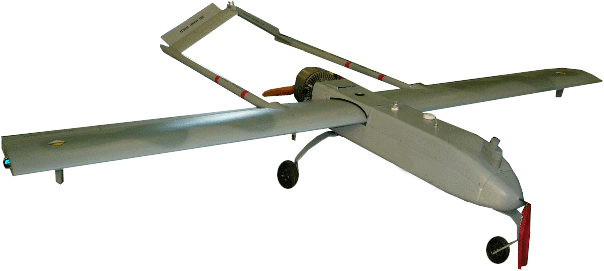
\includegraphics[width=\linewidth]{UAV_RQ7}
                \caption{RQ-7A Shadow 200, разведывательный}
                \label{fig:UAV_RQ7}
        \end{subfigure}
        \caption{Примеры существующих БПЛА}\label{fig:UAVs}
\end{figure}

Для достижения многих практических целей (воздушные разведка и наблюдение, обеспечение связи и мониторинг состояния, доставка и десантирование грузов и другие) использование беспилотных летательных аппаратов может обеспечить преимущество в стоимости эксплуатации и в достижении технических показателей по сравнению с пилотируемыми ЛА. Это связано с тем обстоятельством, что беспилотные ЛА проектируются с учетом менее жестких требований и ограничений, чем пилотируемые ЛА, в частности для них:

\begin{itemize}
\item могут быть установлены иные требования по безопасности конструкции;
\item не требуется систем поддержания работоспособности и жизнеобеспечения экипажа;
\item могут быть сняты ограничения на некоторые режимы полета.
\end{itemize} 

%При их создании особое внимание уделяется требованиям малозаметности и увеличения аэродинамического качества, и как следствие, возможности барражировать в течение длительного времени. 


Благодаря этому БПЛА имеют большой потенциал для разработки для них легких и дешевых конструкций планера, что позволяет успешно решать многие технические задачи, недоступные для пилотируемых летательных аппаратов.




%Рассказать про беспилотник (типы, картинки), предназначены для решения ряда задач.

%Дальше про разные типы.


Как было сказано выше, одной из основных задач беспилотных самолетов является воздушные разведка и наблюдение. Такие самолеты предназначены для продолжительного (до 36 часов для RQ-4 ``Global Hawk'') барражирования без дозаправки, что накладывает на конструкцию самолета высокие требования к весовой эффективности и к аэродинамическому качеству.

%Основное - мониторинг (военный, гражданский). Из этого следуют требования малозаметности и весовой эффективности.

%Использование беспилотника может обеспечить преимущество по сравнению с пилотируемыми, почему.

%Показать несколько существующих и разрабатываемых БПЛА для мониторинга.

Для БПЛА, предназначенных для выполнения военных задач, большую роль также играет малозаметность БПЛА. Требования высоких аэродинамических характеристик и малозаметности накладывают на конструкцию БПЛА ряд ограничений на геометрические параметры; в частности конструкция БПЛА должна иметь минимально возможную строительную высоту, а также иметь обтекаемые обводы. (примеры таких БПЛА приведены на Рис.\ref{fig:UAVs_stealth}). Для достижения высокого аэродинамического качества конструкции таких ЛА должны иметь крыло большого удлинения, интегрированное с несущим фюзеляжем. Однако использование крыльев большого удлинения неизменно влечет за собой появление больших изгибающих моментов в корневой части крыла и в центроплане. 


\begin{figure}[ht]
        \begin{subfigure}[b]{0.47\textwidth}
                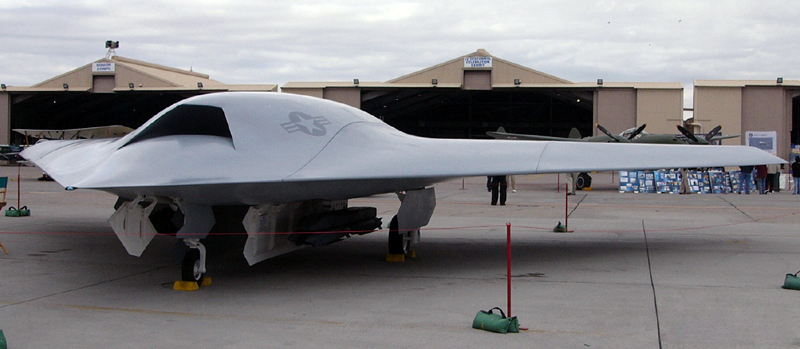
\includegraphics[width=\linewidth]{UAV_X45}
                \caption{Boeing X-45C, экспериментальный многоцелевой}
%http://ru.wikipedia.org/wiki/Boeing_X-45
                \label{fig:UAV_X45}
        \end{subfigure}%
        \hspace{\fill}
        \begin{subfigure}[b]{0.47\textwidth}
                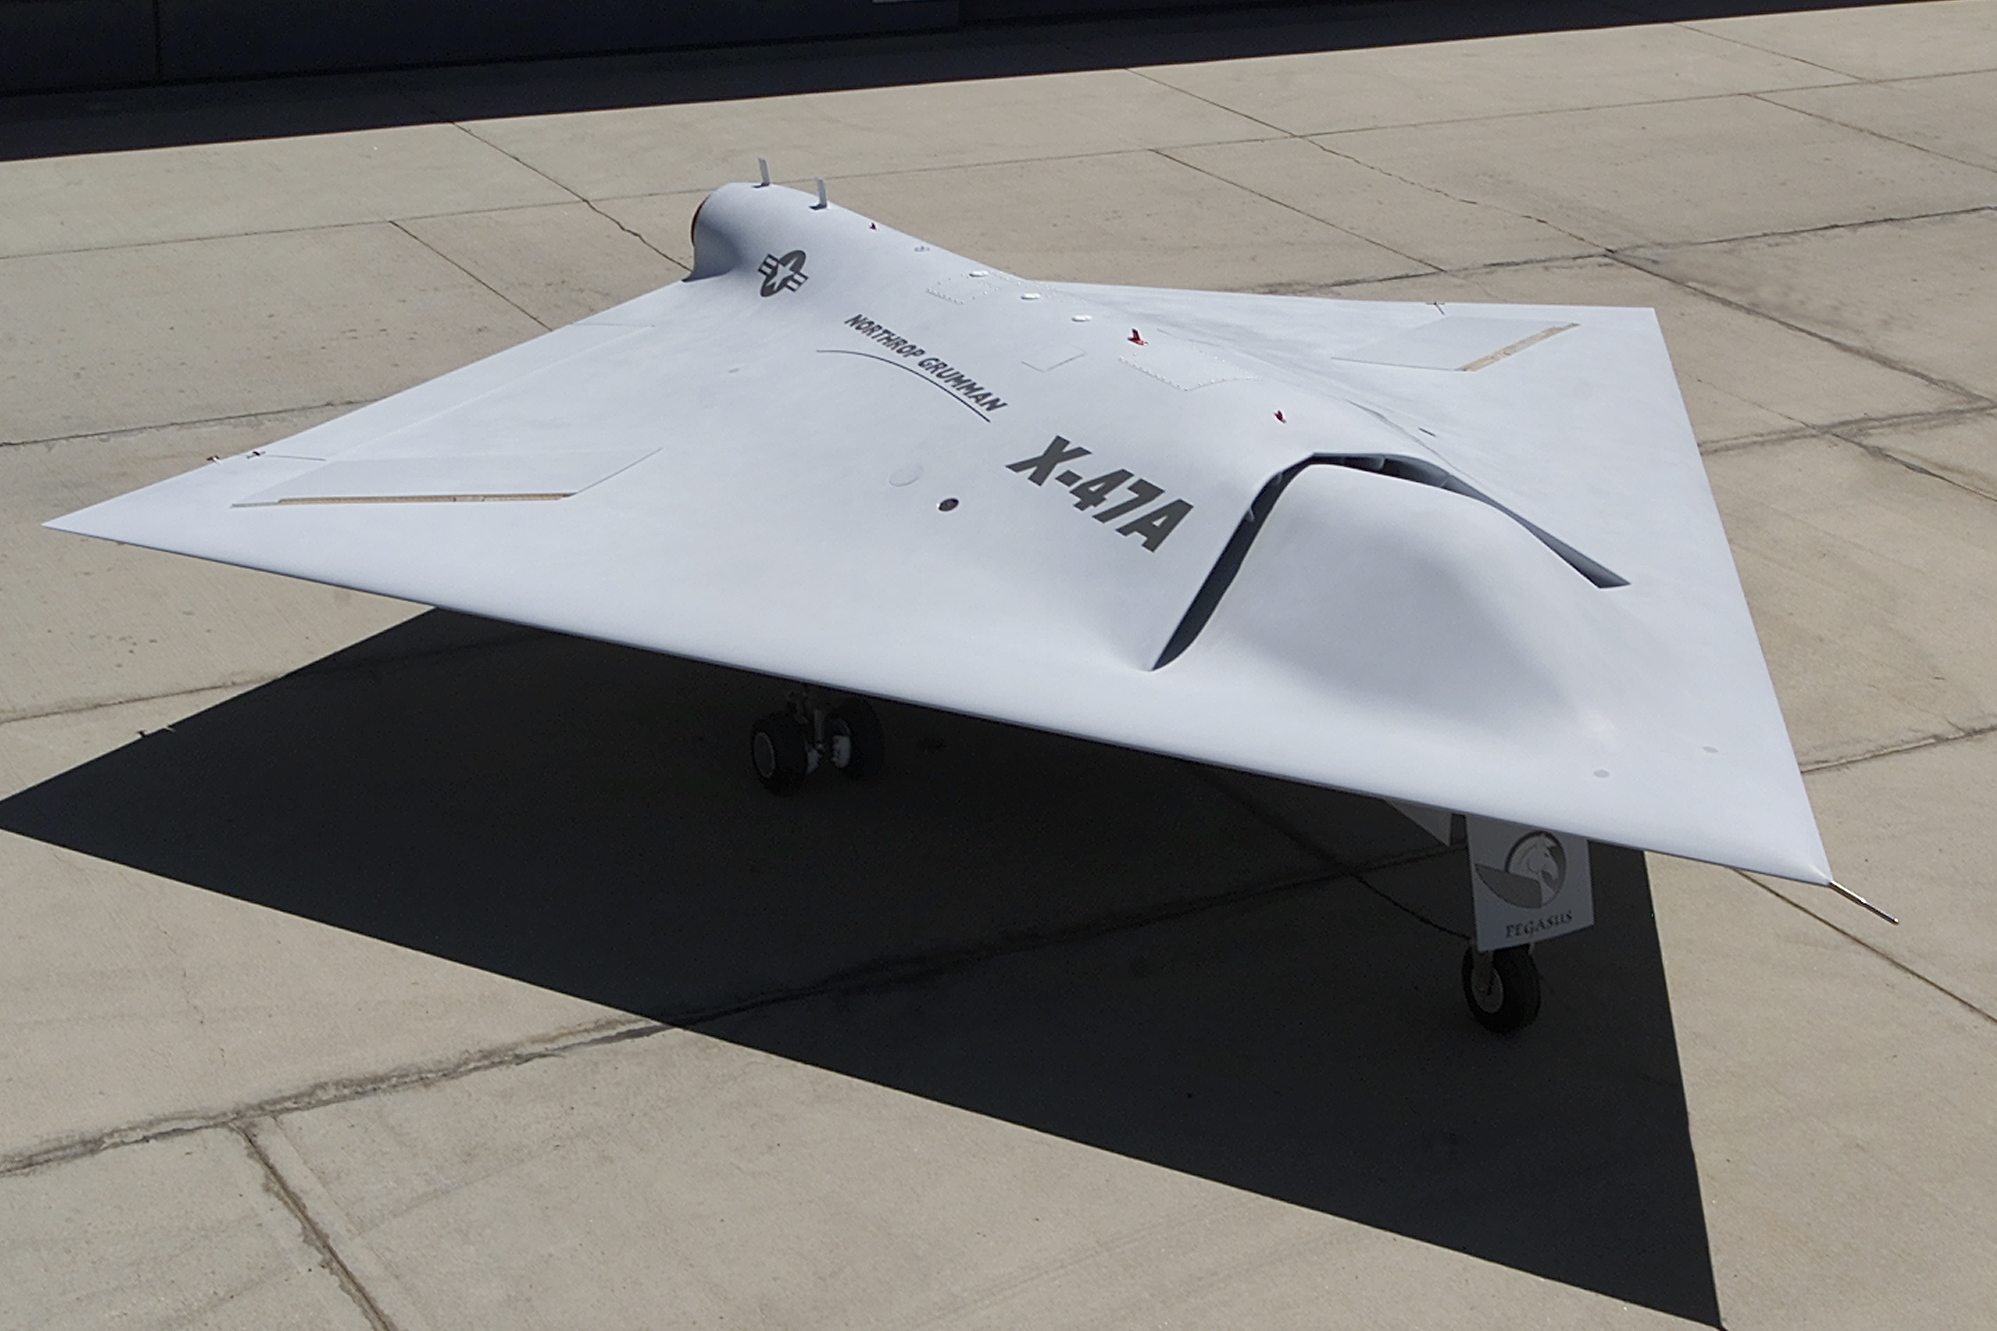
\includegraphics[width=\linewidth]{UAV_X47}
                \caption{Northrop X-47A, боевой} %http://ru.wikipedia.org/wiki/X-47_Pegasus
%		%http://archive.darpa.mil/j-ucas/X-47/gallery/X-47A/hi_res/pegasus2_hi-res.jpg
                \label{fig:UAV_X47}
        \end{subfigure}%
        \caption{БПЛА, выполненные по схеме ``Стелс''}\label{fig:UAVs_stealth}
\end{figure}
%Объясняем, почему нужна интегральная схема и крыло большого удлинения. Цель - меньше заметности следовательно уменьшение строительной высоты, больше аэродинамического качество.

Необходимость уменьшения строительной высоты БПЛА в свою очередь приводит к возникновению проблемы обеспечения высокой степени интеграции двигателя и центроплана. 

Одним из вариантов решения такой интеграционной задачи может служить компоновочная схема БПЛА-ЦАГИ, разработанная в НИО-10, в которой двигатель с воздухозаборником максимально утоплен в конструкции корпуса БПЛА.
На Рис.\ref{fig:BPS} показана центральная часть (кабина) данного ЛА. Компоновку БПЛА-ЦАГИ отличают хорошие аэродинамические характеристики и низкие характеристики заметности \cite{BPS_Report}. Из рисунка видно, что при создании такой компоновочной схемы разработчикам пришлось отказаться от традиционной конструкции центроплана с постоянным поперечным сечением в пользу изогнутого центроплана с переменным поперечным сечением.


\begin{figure}[ht]
\centering
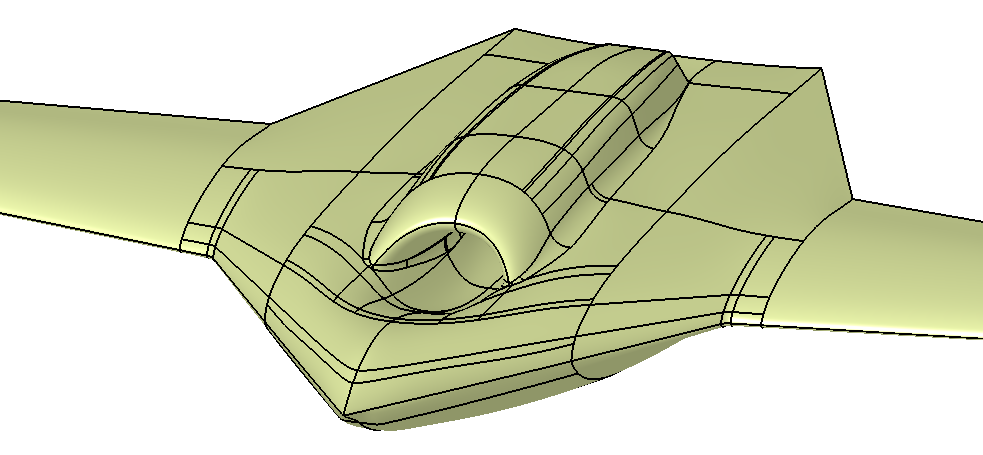
\includegraphics[width=0.8\textwidth]{BPS_Catia}
\caption{Компоновочная схема БПЛА-ЦАГИ}
\label{fig:BPS}
\end{figure}


%Выходим на основную проблему. Проблема интеграции двигателя и центроплана. Описанные выше требования приводят к проблемам. 

%Показываем наш БПЛА (модель из катьи), одним из решений является изогнутый центроплан.



\begin{figure}[ht]
\captionsetup{justification=centering}
\centering
%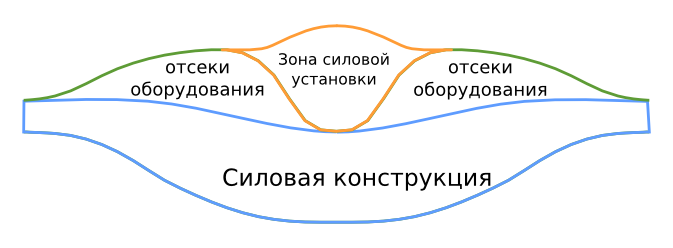
\includegraphics[width=\textwidth]{OriginalSectionWithEngine}
%LaTeX with PSTricks extensions
%%Creator: inkscape 0.48.4
%%Please note this file requires PSTricks extensions
\psset{xunit=.5pt,yunit=.5pt,runit=.5pt}
\begin{pspicture}(1300,600)
{
\newrgbcolor{curcolor}{0.50196081 0.50196081 0.50196081}
\pscustom[linewidth=1,linecolor=curcolor,linestyle=dashed,dash=2 4]
{
\newpath
\moveto(94.3,127.2)
\lineto(1234.6,127.2)
\lineto(1234.61,127.2)
}
}
{
\newrgbcolor{curcolor}{0.50196081 0.50196081 0.50196081}
\pscustom[linewidth=1,linecolor=curcolor]
{
\newpath
\moveto(94.3,127.2)
\lineto(103.3,127.2)
\moveto(1234.6,127.2)
\lineto(1225.6,127.2)
\lineto(1225.61,127.2)
}
}
{
\newrgbcolor{curcolor}{0.50196081 0.50196081 0.50196081}
\pscustom[linestyle=none,fillstyle=solid,fillcolor=curcolor]
{
\newpath
\moveto(73.30712891,126.0984375)
\lineto(73.30712891,127.2703125)
\lineto(76.96923828,127.2703125)
\lineto(76.96923828,126.0984375)
\lineto(73.30712891,126.0984375)
}
}
{
\newrgbcolor{curcolor}{0.50196081 0.50196081 0.50196081}
\pscustom[linestyle=none,fillstyle=solid,fillcolor=curcolor]
{
\newpath
\moveto(78.79296875,122.7)
\lineto(78.79296875,123.82060547)
\lineto(81.42236328,123.82060547)
\lineto(81.42236328,131.76005859)
\lineto(79.09326172,130.09746094)
\lineto(79.09326172,131.34257812)
\lineto(81.53222656,133.01982422)
\lineto(82.74804688,133.01982422)
\lineto(82.74804688,123.82060547)
\lineto(85.26025391,123.82060547)
\lineto(85.26025391,122.7)
\lineto(78.79296875,122.7)
}
}
{
\newrgbcolor{curcolor}{0.50196081 0.50196081 0.50196081}
\pscustom[linewidth=1,linecolor=curcolor,linestyle=dashed,dash=2 4]
{
\newpath
\moveto(94.3,241.2)
\lineto(1234.6,241.2)
\lineto(1234.61,241.2)
}
}
{
\newrgbcolor{curcolor}{0.50196081 0.50196081 0.50196081}
\pscustom[linewidth=1,linecolor=curcolor]
{
\newpath
\moveto(94.3,241.2)
\lineto(103.3,241.2)
\moveto(1234.6,241.2)
\lineto(1225.6,241.2)
\lineto(1225.61,241.2)
}
}
{
\newrgbcolor{curcolor}{0.50196081 0.50196081 0.50196081}
\pscustom[linestyle=none,fillstyle=solid,fillcolor=curcolor]
{
\newpath
\moveto(60.79736328,240.0984375)
\lineto(60.79736328,241.2703125)
\lineto(64.45947266,241.2703125)
\lineto(64.45947266,240.0984375)
\lineto(60.79736328,240.0984375)
}
}
{
\newrgbcolor{curcolor}{0.50196081 0.50196081 0.50196081}
\pscustom[linestyle=none,fillstyle=solid,fillcolor=curcolor]
{
\newpath
\moveto(72.89697266,241.86357422)
\curveto(72.8969649,240.87235911)(72.80175015,240.03739901)(72.61132812,239.35869141)
\curveto(72.42577396,238.6848613)(72.16942656,238.13798684)(71.84228516,237.71806641)
\curveto(71.52001315,237.30302674)(71.13915416,237.00517548)(70.69970703,236.82451172)
\curveto(70.26024879,236.64384771)(69.79149926,236.55351577)(69.29345703,236.55351562)
\curveto(68.79052369,236.55351577)(68.32177416,236.64384771)(67.88720703,236.82451172)
\curveto(67.45263441,237.00517548)(67.07421682,237.30302674)(66.75195312,237.71806641)
\curveto(66.43456902,238.13310404)(66.18310443,238.67753708)(65.99755859,239.35136719)
\curveto(65.81689385,240.03007479)(65.72656191,240.8674763)(65.7265625,241.86357422)
\curveto(65.72656191,242.90360708)(65.81689385,243.76298122)(65.99755859,244.44169922)
\curveto(66.18310443,245.12528454)(66.43701042,245.66971759)(66.75927734,246.075)
\curveto(67.08154103,246.48026366)(67.46240002,246.7634665)(67.90185547,246.92460937)
\curveto(68.34130539,247.09061461)(68.81982054,247.17362234)(69.33740234,247.17363281)
\curveto(69.83056172,247.17362234)(70.29198704,247.09061461)(70.72167969,246.92460937)
\curveto(71.15624398,246.7634665)(71.53466157,246.48026366)(71.85693359,246.075)
\curveto(72.17919218,245.66971759)(72.43309818,245.12528454)(72.61865234,244.44169922)
\curveto(72.80419156,243.76298122)(72.8969649,242.90360708)(72.89697266,241.86357422)
\moveto(71.55664062,241.86357422)
\curveto(71.55663421,242.68388073)(71.50780613,243.3650324)(71.41015625,243.90703125)
\curveto(71.31249383,244.4538985)(71.168451,244.88846837)(70.97802734,245.21074219)
\curveto(70.78759201,245.53788179)(70.55321724,245.76737375)(70.27490234,245.89921875)
\curveto(70.00145998,246.03592816)(69.6889603,246.10428747)(69.33740234,246.10429687)
\curveto(68.96630477,246.10428747)(68.63915666,246.03592816)(68.35595703,245.89921875)
\curveto(68.07275097,245.76249094)(67.8334934,245.53055758)(67.63818359,245.20341797)
\curveto(67.4477516,244.88114416)(67.30370877,244.44657428)(67.20605469,243.89970703)
\curveto(67.10839647,243.35770819)(67.05956839,242.67899793)(67.05957031,241.86357422)
\curveto(67.05956839,241.07255422)(67.10839647,240.40605098)(67.20605469,239.8640625)
\curveto(67.30859158,239.32206769)(67.45507581,238.88505641)(67.64550781,238.55302734)
\curveto(67.84081761,238.22587738)(68.07763378,237.98906121)(68.35595703,237.84257812)
\curveto(68.63427385,237.70097556)(68.95165635,237.63017485)(69.30810547,237.63017578)
\curveto(69.65478064,237.63017485)(69.96728033,237.70097556)(70.24560547,237.84257812)
\curveto(70.5239204,237.98906121)(70.75829516,238.22587738)(70.94873047,238.55302734)
\curveto(71.14403697,238.88505641)(71.2929626,239.32206769)(71.39550781,239.8640625)
\curveto(71.50292333,240.40605098)(71.55663421,241.07255422)(71.55664062,241.86357422)
}
}
{
\newrgbcolor{curcolor}{0.50196081 0.50196081 0.50196081}
\pscustom[linestyle=none,fillstyle=solid,fillcolor=curcolor]
{
\newpath
\moveto(74.85986328,236.7)
\lineto(74.85986328,238.30400391)
\lineto(76.28808594,238.30400391)
\lineto(76.28808594,236.7)
\lineto(74.85986328,236.7)
}
}
{
\newrgbcolor{curcolor}{0.50196081 0.50196081 0.50196081}
\pscustom[linestyle=none,fillstyle=solid,fillcolor=curcolor]
{
\newpath
\moveto(85.36279297,240.06181641)
\curveto(85.36278526,239.54423544)(85.28466033,239.0706031)(85.12841797,238.64091797)
\curveto(84.97216065,238.21122896)(84.74022729,237.84013558)(84.43261719,237.52763672)
\curveto(84.12499353,237.22001901)(83.74169313,236.98076144)(83.28271484,236.80986328)
\curveto(82.8286081,236.6389649)(82.30126488,236.55351577)(81.70068359,236.55351562)
\curveto(81.1586879,236.55351577)(80.68505556,236.61699227)(80.27978516,236.74394531)
\curveto(79.8793923,236.87089827)(79.54003717,237.04423794)(79.26171875,237.26396484)
\curveto(78.9833971,237.48857343)(78.76122936,237.74980364)(78.59521484,238.04765625)
\curveto(78.43408125,238.34550617)(78.31933527,238.66533007)(78.25097656,239.00712891)
\lineto(79.58398438,239.1609375)
\curveto(79.63769333,238.96562273)(79.71337684,238.77519324)(79.81103516,238.58964844)
\curveto(79.90868915,238.40898267)(80.04052495,238.24540861)(80.20654297,238.09892578)
\curveto(80.37743868,237.95732296)(80.584958,237.84257698)(80.82910156,237.7546875)
\curveto(81.07812157,237.67167872)(81.37841424,237.63017485)(81.72998047,237.63017578)
\curveto(82.07177292,237.63017485)(82.38183121,237.68144433)(82.66015625,237.78398437)
\curveto(82.93847127,237.89140506)(83.17528744,238.0476549)(83.37060547,238.25273437)
\curveto(83.57079486,238.45781074)(83.7246033,238.70927533)(83.83203125,239.00712891)
\curveto(83.93944684,239.30497786)(83.99315772,239.6467744)(83.99316406,240.03251953)
\curveto(83.99315772,240.34989869)(83.94188824,240.64042575)(83.83935547,240.90410156)
\curveto(83.73681032,241.17265178)(83.59032609,241.40214374)(83.39990234,241.59257812)
\curveto(83.2094671,241.78788554)(82.97509233,241.93925257)(82.69677734,242.04667969)
\curveto(82.42333507,242.15409611)(82.11083538,242.20780699)(81.75927734,242.2078125)
\curveto(81.53954689,242.20780699)(81.33691038,242.18827576)(81.15136719,242.14921875)
\curveto(80.965817,242.11015084)(80.79247733,242.05643996)(80.63134766,241.98808594)
\curveto(80.47509483,241.91972134)(80.33105201,241.83915502)(80.19921875,241.74638672)
\curveto(80.0722632,241.65849114)(79.95263442,241.56571779)(79.84033203,241.46806641)
\lineto(78.55126953,241.46806641)
\lineto(78.89550781,247.01982422)
\lineto(84.76220703,247.01982422)
\lineto(84.76220703,245.89921875)
\lineto(80.09667969,245.89921875)
\lineto(79.89892578,242.62529297)
\curveto(80.1332983,242.80595093)(80.42626676,242.95975937)(80.77783203,243.08671875)
\curveto(81.12939105,243.21854817)(81.5468711,243.28446607)(82.03027344,243.28447266)
\curveto(82.54296386,243.28446607)(83.00438918,243.20634115)(83.41455078,243.05009766)
\curveto(83.82470086,242.89384146)(84.1738216,242.67167372)(84.46191406,242.38359375)
\curveto(84.7499929,242.10038522)(84.97216065,241.7610301)(85.12841797,241.36552734)
\curveto(85.28466033,240.97001526)(85.36278526,240.53544538)(85.36279297,240.06181641)
}
}
{
\newrgbcolor{curcolor}{0.50196081 0.50196081 0.50196081}
\pscustom[linewidth=1,linecolor=curcolor,linestyle=dashed,dash=2 4]
{
\newpath
\moveto(94.3,355.3)
\lineto(1234.6,355.3)
\lineto(1234.61,355.3)
}
}
{
\newrgbcolor{curcolor}{0.50196081 0.50196081 0.50196081}
\pscustom[linewidth=1,linecolor=curcolor]
{
\newpath
\moveto(94.3,355.3)
\lineto(103.3,355.3)
\moveto(1234.6,355.3)
\lineto(1225.6,355.3)
\lineto(1225.61,355.3)
}
}
{
\newrgbcolor{curcolor}{0.50196081 0.50196081 0.50196081}
\pscustom[linestyle=none,fillstyle=solid,fillcolor=curcolor]
{
\newpath
\moveto(85.40673828,355.96357422)
\curveto(85.40673052,354.97235911)(85.31151578,354.13739901)(85.12109375,353.45869141)
\curveto(84.93553959,352.7848613)(84.67919219,352.23798684)(84.35205078,351.81806641)
\curveto(84.02977878,351.40302674)(83.64891978,351.10517548)(83.20947266,350.92451172)
\curveto(82.77001441,350.74384771)(82.30126488,350.65351577)(81.80322266,350.65351563)
\curveto(81.30028932,350.65351577)(80.83153979,350.74384771)(80.39697266,350.92451172)
\curveto(79.96240003,351.10517548)(79.58398244,351.40302674)(79.26171875,351.81806641)
\curveto(78.94433464,352.23310404)(78.69287005,352.77753708)(78.50732422,353.45136719)
\curveto(78.32665948,354.13007479)(78.23632754,354.9674763)(78.23632812,355.96357422)
\curveto(78.23632754,357.00360708)(78.32665948,357.86298122)(78.50732422,358.54169922)
\curveto(78.69287005,359.22528454)(78.94677605,359.76971759)(79.26904297,360.175)
\curveto(79.59130665,360.58026366)(79.97216565,360.8634665)(80.41162109,361.02460938)
\curveto(80.85107102,361.19061461)(81.32958616,361.27362234)(81.84716797,361.27363281)
\curveto(82.34032734,361.27362234)(82.80175266,361.19061461)(83.23144531,361.02460938)
\curveto(83.66600961,360.8634665)(84.0444272,360.58026366)(84.36669922,360.175)
\curveto(84.68895781,359.76971759)(84.9428638,359.22528454)(85.12841797,358.54169922)
\curveto(85.31395718,357.86298122)(85.40673052,357.00360708)(85.40673828,355.96357422)
\moveto(84.06640625,355.96357422)
\curveto(84.06639983,356.78388073)(84.01757176,357.4650324)(83.91992188,358.00703125)
\curveto(83.82225945,358.5538985)(83.67821663,358.98846837)(83.48779297,359.31074219)
\curveto(83.29735763,359.63788179)(83.06298287,359.86737375)(82.78466797,359.99921875)
\curveto(82.51122561,360.13592816)(82.19872592,360.20428747)(81.84716797,360.20429688)
\curveto(81.47607039,360.20428747)(81.14892228,360.13592816)(80.86572266,359.99921875)
\curveto(80.5825166,359.86249094)(80.34325903,359.63055758)(80.14794922,359.30341797)
\curveto(79.95751722,358.98114416)(79.8134744,358.54657428)(79.71582031,357.99970703)
\curveto(79.61816209,357.45770819)(79.56933402,356.77899793)(79.56933594,355.96357422)
\curveto(79.56933402,355.17255422)(79.61816209,354.50605098)(79.71582031,353.9640625)
\curveto(79.81835721,353.42206769)(79.96484144,352.98505641)(80.15527344,352.65302734)
\curveto(80.35058324,352.32587738)(80.58739941,352.08906121)(80.86572266,351.94257813)
\curveto(81.14403948,351.80097556)(81.46142197,351.73017485)(81.81787109,351.73017578)
\curveto(82.16454627,351.73017485)(82.47704595,351.80097556)(82.75537109,351.94257813)
\curveto(83.03368602,352.08906121)(83.26806079,352.32587738)(83.45849609,352.65302734)
\curveto(83.65380259,352.98505641)(83.80272822,353.42206769)(83.90527344,353.9640625)
\curveto(84.01268895,354.50605098)(84.06639983,355.17255422)(84.06640625,355.96357422)
}
}
{
\newrgbcolor{curcolor}{0.50196081 0.50196081 0.50196081}
\pscustom[linewidth=1,linecolor=curcolor,linestyle=dashed,dash=2 4]
{
\newpath
\moveto(94.3,469.3)
\lineto(1234.6,469.3)
\lineto(1234.61,469.3)
}
}
{
\newrgbcolor{curcolor}{0.50196081 0.50196081 0.50196081}
\pscustom[linewidth=1,linecolor=curcolor]
{
\newpath
\moveto(94.3,469.3)
\lineto(103.3,469.3)
\moveto(1234.6,469.3)
\lineto(1225.6,469.3)
\lineto(1225.61,469.3)
}
}
{
\newrgbcolor{curcolor}{0.50196081 0.50196081 0.50196081}
\pscustom[linestyle=none,fillstyle=solid,fillcolor=curcolor]
{
\newpath
\moveto(72.89697266,469.96357422)
\curveto(72.8969649,468.97235911)(72.80175015,468.13739901)(72.61132812,467.45869141)
\curveto(72.42577396,466.7848613)(72.16942656,466.23798684)(71.84228516,465.81806641)
\curveto(71.52001315,465.40302674)(71.13915416,465.10517548)(70.69970703,464.92451172)
\curveto(70.26024879,464.74384771)(69.79149926,464.65351577)(69.29345703,464.65351563)
\curveto(68.79052369,464.65351577)(68.32177416,464.74384771)(67.88720703,464.92451172)
\curveto(67.45263441,465.10517548)(67.07421682,465.40302674)(66.75195312,465.81806641)
\curveto(66.43456902,466.23310404)(66.18310443,466.77753708)(65.99755859,467.45136719)
\curveto(65.81689385,468.13007479)(65.72656191,468.9674763)(65.7265625,469.96357422)
\curveto(65.72656191,471.00360708)(65.81689385,471.86298122)(65.99755859,472.54169922)
\curveto(66.18310443,473.22528454)(66.43701042,473.76971759)(66.75927734,474.175)
\curveto(67.08154103,474.58026366)(67.46240002,474.8634665)(67.90185547,475.02460938)
\curveto(68.34130539,475.19061461)(68.81982054,475.27362234)(69.33740234,475.27363281)
\curveto(69.83056172,475.27362234)(70.29198704,475.19061461)(70.72167969,475.02460938)
\curveto(71.15624398,474.8634665)(71.53466157,474.58026366)(71.85693359,474.175)
\curveto(72.17919218,473.76971759)(72.43309818,473.22528454)(72.61865234,472.54169922)
\curveto(72.80419156,471.86298122)(72.8969649,471.00360708)(72.89697266,469.96357422)
\moveto(71.55664062,469.96357422)
\curveto(71.55663421,470.78388073)(71.50780613,471.4650324)(71.41015625,472.00703125)
\curveto(71.31249383,472.5538985)(71.168451,472.98846837)(70.97802734,473.31074219)
\curveto(70.78759201,473.63788179)(70.55321724,473.86737375)(70.27490234,473.99921875)
\curveto(70.00145998,474.13592816)(69.6889603,474.20428747)(69.33740234,474.20429688)
\curveto(68.96630477,474.20428747)(68.63915666,474.13592816)(68.35595703,473.99921875)
\curveto(68.07275097,473.86249094)(67.8334934,473.63055758)(67.63818359,473.30341797)
\curveto(67.4477516,472.98114416)(67.30370877,472.54657428)(67.20605469,471.99970703)
\curveto(67.10839647,471.45770819)(67.05956839,470.77899793)(67.05957031,469.96357422)
\curveto(67.05956839,469.17255422)(67.10839647,468.50605098)(67.20605469,467.9640625)
\curveto(67.30859158,467.42206769)(67.45507581,466.98505641)(67.64550781,466.65302734)
\curveto(67.84081761,466.32587738)(68.07763378,466.08906121)(68.35595703,465.94257813)
\curveto(68.63427385,465.80097556)(68.95165635,465.73017485)(69.30810547,465.73017578)
\curveto(69.65478064,465.73017485)(69.96728033,465.80097556)(70.24560547,465.94257813)
\curveto(70.5239204,466.08906121)(70.75829516,466.32587738)(70.94873047,466.65302734)
\curveto(71.14403697,466.98505641)(71.2929626,467.42206769)(71.39550781,467.9640625)
\curveto(71.50292333,468.50605098)(71.55663421,469.17255422)(71.55664062,469.96357422)
}
}
{
\newrgbcolor{curcolor}{0.50196081 0.50196081 0.50196081}
\pscustom[linestyle=none,fillstyle=solid,fillcolor=curcolor]
{
\newpath
\moveto(74.85986328,464.8)
\lineto(74.85986328,466.40400391)
\lineto(76.28808594,466.40400391)
\lineto(76.28808594,464.8)
\lineto(74.85986328,464.8)
}
}
{
\newrgbcolor{curcolor}{0.50196081 0.50196081 0.50196081}
\pscustom[linestyle=none,fillstyle=solid,fillcolor=curcolor]
{
\newpath
\moveto(85.36279297,468.16181641)
\curveto(85.36278526,467.64423544)(85.28466033,467.1706031)(85.12841797,466.74091797)
\curveto(84.97216065,466.31122896)(84.74022729,465.94013558)(84.43261719,465.62763672)
\curveto(84.12499353,465.32001901)(83.74169313,465.08076144)(83.28271484,464.90986328)
\curveto(82.8286081,464.7389649)(82.30126488,464.65351577)(81.70068359,464.65351563)
\curveto(81.1586879,464.65351577)(80.68505556,464.71699227)(80.27978516,464.84394531)
\curveto(79.8793923,464.97089827)(79.54003717,465.14423794)(79.26171875,465.36396484)
\curveto(78.9833971,465.58857343)(78.76122936,465.84980364)(78.59521484,466.14765625)
\curveto(78.43408125,466.44550617)(78.31933527,466.76533007)(78.25097656,467.10712891)
\lineto(79.58398438,467.2609375)
\curveto(79.63769333,467.06562273)(79.71337684,466.87519324)(79.81103516,466.68964844)
\curveto(79.90868915,466.50898267)(80.04052495,466.34540861)(80.20654297,466.19892578)
\curveto(80.37743868,466.05732296)(80.584958,465.94257698)(80.82910156,465.8546875)
\curveto(81.07812157,465.77167872)(81.37841424,465.73017485)(81.72998047,465.73017578)
\curveto(82.07177292,465.73017485)(82.38183121,465.78144433)(82.66015625,465.88398438)
\curveto(82.93847127,465.99140506)(83.17528744,466.1476549)(83.37060547,466.35273438)
\curveto(83.57079486,466.55781074)(83.7246033,466.80927533)(83.83203125,467.10712891)
\curveto(83.93944684,467.40497786)(83.99315772,467.7467744)(83.99316406,468.13251953)
\curveto(83.99315772,468.44989869)(83.94188824,468.74042575)(83.83935547,469.00410156)
\curveto(83.73681032,469.27265178)(83.59032609,469.50214374)(83.39990234,469.69257813)
\curveto(83.2094671,469.88788554)(82.97509233,470.03925257)(82.69677734,470.14667969)
\curveto(82.42333507,470.25409611)(82.11083538,470.30780699)(81.75927734,470.3078125)
\curveto(81.53954689,470.30780699)(81.33691038,470.28827576)(81.15136719,470.24921875)
\curveto(80.965817,470.21015084)(80.79247733,470.15643996)(80.63134766,470.08808594)
\curveto(80.47509483,470.01972134)(80.33105201,469.93915502)(80.19921875,469.84638672)
\curveto(80.0722632,469.75849114)(79.95263442,469.66571779)(79.84033203,469.56806641)
\lineto(78.55126953,469.56806641)
\lineto(78.89550781,475.11982422)
\lineto(84.76220703,475.11982422)
\lineto(84.76220703,473.99921875)
\lineto(80.09667969,473.99921875)
\lineto(79.89892578,470.72529297)
\curveto(80.1332983,470.90595093)(80.42626676,471.05975937)(80.77783203,471.18671875)
\curveto(81.12939105,471.31854817)(81.5468711,471.38446607)(82.03027344,471.38447266)
\curveto(82.54296386,471.38446607)(83.00438918,471.30634115)(83.41455078,471.15009766)
\curveto(83.82470086,470.99384146)(84.1738216,470.77167372)(84.46191406,470.48359375)
\curveto(84.7499929,470.20038522)(84.97216065,469.8610301)(85.12841797,469.46552734)
\curveto(85.28466033,469.07001526)(85.36278526,468.63544538)(85.36279297,468.16181641)
}
}
{
\newrgbcolor{curcolor}{0.50196081 0.50196081 0.50196081}
\pscustom[linewidth=1,linecolor=curcolor,linestyle=dashed,dash=2 4]
{
\newpath
\moveto(94.3,583.3)
\lineto(1234.6,583.3)
\lineto(1234.61,583.3)
}
}
{
\newrgbcolor{curcolor}{0.50196081 0.50196081 0.50196081}
\pscustom[linewidth=1,linecolor=curcolor]
{
\newpath
\moveto(94.3,583.3)
\lineto(103.3,583.3)
\moveto(1234.6,583.3)
\lineto(1225.6,583.3)
\lineto(1225.61,583.3)
}
}
{
\newrgbcolor{curcolor}{0.50196081 0.50196081 0.50196081}
\pscustom[linestyle=none,fillstyle=solid,fillcolor=curcolor]
{
\newpath
\moveto(78.79296875,578.8)
\lineto(78.79296875,579.92060547)
\lineto(81.42236328,579.92060547)
\lineto(81.42236328,587.86005859)
\lineto(79.09326172,586.19746094)
\lineto(79.09326172,587.44257812)
\lineto(81.53222656,589.11982422)
\lineto(82.74804688,589.11982422)
\lineto(82.74804688,579.92060547)
\lineto(85.26025391,579.92060547)
\lineto(85.26025391,578.8)
\lineto(78.79296875,578.8)
}
}
{
\newrgbcolor{curcolor}{0.50196081 0.50196081 0.50196081}
\pscustom[linewidth=1,linecolor=curcolor,linestyle=dashed,dash=2 4]
{
\newpath
\moveto(208.3,36)
\lineto(208.3,583.3)
\lineto(208.31,583.3)
}
}
{
\newrgbcolor{curcolor}{0.50196081 0.50196081 0.50196081}
\pscustom[linewidth=1,linecolor=curcolor]
{
\newpath
\moveto(208.3,36)
\lineto(208.3,45)
\moveto(208.3,583.3)
\lineto(208.3,574.3)
\lineto(208.31,574.3)
}
}
{
\newrgbcolor{curcolor}{0.50196081 0.50196081 0.50196081}
\pscustom[linestyle=none,fillstyle=solid,fillcolor=curcolor]
{
\newpath
\moveto(202.28681641,16.8984375)
\lineto(202.28681641,18.0703125)
\lineto(205.94892578,18.0703125)
\lineto(205.94892578,16.8984375)
\lineto(202.28681641,16.8984375)
}
}
{
\newrgbcolor{curcolor}{0.50196081 0.50196081 0.50196081}
\pscustom[linestyle=none,fillstyle=solid,fillcolor=curcolor]
{
\newpath
\moveto(207.38447266,13.5)
\lineto(207.38447266,14.43017578)
\curveto(207.63349509,15.00146334)(207.93622916,15.50439253)(208.29267578,15.93896484)
\curveto(208.65400188,16.37841509)(209.03241947,16.77392251)(209.42792969,17.12548828)
\curveto(209.82343431,17.48192961)(210.21405892,17.81151913)(210.59980469,18.11425781)
\curveto(210.99042533,18.41698727)(211.34198748,18.71972134)(211.65449219,19.02246094)
\curveto(211.96698685,19.32518949)(212.21845144,19.64257198)(212.40888672,19.97460938)
\curveto(212.60419324,20.30663382)(212.7018494,20.68261)(212.70185547,21.10253906)
\curveto(212.7018494,21.39549992)(212.65790413,21.65184732)(212.57001953,21.87158203)
\curveto(212.48212305,22.09618281)(212.35517006,22.2841709)(212.18916016,22.43554688)
\curveto(212.02313914,22.58690498)(211.82294403,22.69920955)(211.58857422,22.77246094)
\curveto(211.3590773,22.85057659)(211.1027299,22.88963905)(210.81953125,22.88964844)
\curveto(210.55585545,22.88963905)(210.30683226,22.85301799)(210.07246094,22.77978516)
\curveto(209.84296554,22.70653376)(209.63788762,22.59667059)(209.45722656,22.45019531)
\curveto(209.27655985,22.30370213)(209.12763422,22.12059685)(209.01044922,21.90087891)
\curveto(208.89814226,21.68602697)(208.82490015,21.43456238)(208.79072266,21.14648438)
\lineto(207.44306641,21.27099609)
\curveto(207.48701086,21.6420817)(207.58954982,21.99120245)(207.75068359,22.31835938)
\curveto(207.91181512,22.64549867)(208.13398287,22.93114291)(208.4171875,23.17529297)
\curveto(208.70038855,23.42430648)(209.03974368,23.61961879)(209.43525391,23.76123047)
\curveto(209.83564133,23.90282163)(210.29706665,23.97362234)(210.81953125,23.97363281)
\curveto(211.33222186,23.97362234)(211.78876437,23.91258724)(212.18916016,23.79052734)
\curveto(212.58954482,23.66844686)(212.92645855,23.48778298)(213.19990234,23.24853516)
\curveto(213.47821581,23.00926783)(213.69061794,22.71385797)(213.83710938,22.36230469)
\curveto(213.9835864,22.01073368)(214.05682851,21.60546064)(214.05683594,21.14648438)
\curveto(214.05682851,20.79979739)(213.99335201,20.47020787)(213.86640625,20.15771484)
\curveto(213.74432882,19.8452085)(213.57831336,19.54735723)(213.36835938,19.26416016)
\curveto(213.16327472,18.98095155)(212.92401714,18.70751432)(212.65058594,18.44384766)
\curveto(212.37714269,18.1801711)(212.09149844,17.9213823)(211.79365234,17.66748047)
\curveto(211.49579592,17.41845311)(211.19550325,17.16942992)(210.89277344,16.92041016)
\curveto(210.5900351,16.67626635)(210.30439086,16.42968457)(210.03583984,16.18066406)
\curveto(209.77216483,15.93163819)(209.53534866,15.6777322)(209.32539063,15.41894531)
\curveto(209.1154272,15.1650374)(208.95185315,14.89892438)(208.83466797,14.62060547)
\lineto(214.21796875,14.62060547)
\lineto(214.21796875,13.5)
\lineto(207.38447266,13.5)
}
}
{
\newrgbcolor{curcolor}{0.50196081 0.50196081 0.50196081}
\pscustom[linewidth=1,linecolor=curcolor,linestyle=dashed,dash=2 4]
{
\newpath
\moveto(436.4,36)
\lineto(436.4,583.3)
\lineto(436.41,583.3)
}
}
{
\newrgbcolor{curcolor}{0.50196081 0.50196081 0.50196081}
\pscustom[linewidth=1,linecolor=curcolor]
{
\newpath
\moveto(436.4,36)
\lineto(436.4,45)
\moveto(436.4,583.3)
\lineto(436.4,574.3)
\lineto(436.41,574.3)
}
}
{
\newrgbcolor{curcolor}{0.50196081 0.50196081 0.50196081}
\pscustom[linestyle=none,fillstyle=solid,fillcolor=curcolor]
{
\newpath
\moveto(430.38681641,16.8984375)
\lineto(430.38681641,18.0703125)
\lineto(434.04892578,18.0703125)
\lineto(434.04892578,16.8984375)
\lineto(430.38681641,16.8984375)
}
}
{
\newrgbcolor{curcolor}{0.50196081 0.50196081 0.50196081}
\pscustom[linestyle=none,fillstyle=solid,fillcolor=curcolor]
{
\newpath
\moveto(435.87265625,13.5)
\lineto(435.87265625,14.62060547)
\lineto(438.50205078,14.62060547)
\lineto(438.50205078,22.56005859)
\lineto(436.17294922,20.89746094)
\lineto(436.17294922,22.14257812)
\lineto(438.61191406,23.81982422)
\lineto(439.82773437,23.81982422)
\lineto(439.82773437,14.62060547)
\lineto(442.33994141,14.62060547)
\lineto(442.33994141,13.5)
\lineto(435.87265625,13.5)
}
}
{
\newrgbcolor{curcolor}{0.50196081 0.50196081 0.50196081}
\pscustom[linewidth=1,linecolor=curcolor,linestyle=dashed,dash=2 4]
{
\newpath
\moveto(664.5,36)
\lineto(664.5,583.3)
\lineto(664.51,583.3)
}
}
{
\newrgbcolor{curcolor}{0.50196081 0.50196081 0.50196081}
\pscustom[linewidth=1,linecolor=curcolor]
{
\newpath
\moveto(664.5,36)
\lineto(664.5,45)
\moveto(664.5,583.3)
\lineto(664.5,574.3)
\lineto(664.51,574.3)
}
}
{
\newrgbcolor{curcolor}{0.50196081 0.50196081 0.50196081}
\pscustom[linestyle=none,fillstyle=solid,fillcolor=curcolor]
{
\newpath
\moveto(668.08154297,18.66357422)
\curveto(668.08153521,17.67235911)(667.98632046,16.83739901)(667.79589844,16.15869141)
\curveto(667.61034428,15.4848613)(667.35399688,14.93798684)(667.02685547,14.51806641)
\curveto(666.70458346,14.10302674)(666.32372447,13.80517548)(665.88427734,13.62451172)
\curveto(665.4448191,13.44384771)(664.97606957,13.35351577)(664.47802734,13.35351562)
\curveto(663.97509401,13.35351577)(663.50634448,13.44384771)(663.07177734,13.62451172)
\curveto(662.63720472,13.80517548)(662.25878713,14.10302674)(661.93652344,14.51806641)
\curveto(661.61913933,14.93310404)(661.36767474,15.47753708)(661.18212891,16.15136719)
\curveto(661.00146417,16.83007479)(660.91113223,17.6674763)(660.91113281,18.66357422)
\curveto(660.91113223,19.70360708)(661.00146417,20.56298122)(661.18212891,21.24169922)
\curveto(661.36767474,21.92528454)(661.62158073,22.46971759)(661.94384766,22.875)
\curveto(662.26611134,23.28026366)(662.64697033,23.5634665)(663.08642578,23.72460938)
\curveto(663.52587571,23.89061461)(664.00439085,23.97362234)(664.52197266,23.97363281)
\curveto(665.01513203,23.97362234)(665.47655735,23.89061461)(665.90625,23.72460938)
\curveto(666.3408143,23.5634665)(666.71923189,23.28026366)(667.04150391,22.875)
\curveto(667.36376249,22.46971759)(667.61766849,21.92528454)(667.80322266,21.24169922)
\curveto(667.98876187,20.56298122)(668.08153521,19.70360708)(668.08154297,18.66357422)
\moveto(666.74121094,18.66357422)
\curveto(666.74120452,19.48388073)(666.69237645,20.1650324)(666.59472656,20.70703125)
\curveto(666.49706414,21.2538985)(666.35302132,21.68846837)(666.16259766,22.01074219)
\curveto(665.97216232,22.33788179)(665.73778756,22.56737375)(665.45947266,22.69921875)
\curveto(665.1860303,22.83592816)(664.87353061,22.90428747)(664.52197266,22.90429688)
\curveto(664.15087508,22.90428747)(663.82372697,22.83592816)(663.54052734,22.69921875)
\curveto(663.25732129,22.56249094)(663.01806371,22.33055758)(662.82275391,22.00341797)
\curveto(662.63232191,21.68114416)(662.48827909,21.24657428)(662.390625,20.69970703)
\curveto(662.29296678,20.15770819)(662.24413871,19.47899793)(662.24414062,18.66357422)
\curveto(662.24413871,17.87255422)(662.29296678,17.20605098)(662.390625,16.6640625)
\curveto(662.49316189,16.12206769)(662.63964612,15.68505641)(662.83007812,15.35302734)
\curveto(663.02538792,15.02587738)(663.26220409,14.78906121)(663.54052734,14.64257812)
\curveto(663.81884416,14.50097556)(664.13622666,14.43017485)(664.49267578,14.43017578)
\curveto(664.83935095,14.43017485)(665.15185064,14.50097556)(665.43017578,14.64257812)
\curveto(665.70849071,14.78906121)(665.94286548,15.02587738)(666.13330078,15.35302734)
\curveto(666.32860728,15.68505641)(666.47753291,16.12206769)(666.58007812,16.6640625)
\curveto(666.68749364,17.20605098)(666.74120452,17.87255422)(666.74121094,18.66357422)
}
}
{
\newrgbcolor{curcolor}{0.50196081 0.50196081 0.50196081}
\pscustom[linewidth=1,linecolor=curcolor,linestyle=dashed,dash=2 4]
{
\newpath
\moveto(892.5,36)
\lineto(892.5,583.3)
\lineto(892.51,583.3)
}
}
{
\newrgbcolor{curcolor}{0.50196081 0.50196081 0.50196081}
\pscustom[linewidth=1,linecolor=curcolor]
{
\newpath
\moveto(892.5,36)
\lineto(892.5,45)
\moveto(892.5,583.3)
\lineto(892.5,574.3)
\lineto(892.51,574.3)
}
}
{
\newrgbcolor{curcolor}{0.50196081 0.50196081 0.50196081}
\pscustom[linestyle=none,fillstyle=solid,fillcolor=curcolor]
{
\newpath
\moveto(889.46777344,13.5)
\lineto(889.46777344,14.62060547)
\lineto(892.09716797,14.62060547)
\lineto(892.09716797,22.56005859)
\lineto(889.76806641,20.89746094)
\lineto(889.76806641,22.14257812)
\lineto(892.20703125,23.81982422)
\lineto(893.42285156,23.81982422)
\lineto(893.42285156,14.62060547)
\lineto(895.93505859,14.62060547)
\lineto(895.93505859,13.5)
\lineto(889.46777344,13.5)
}
}
{
\newrgbcolor{curcolor}{0.50196081 0.50196081 0.50196081}
\pscustom[linewidth=1,linecolor=curcolor,linestyle=dashed,dash=2 4]
{
\newpath
\moveto(1120.6,36)
\lineto(1120.6,538.3)
\moveto(1120.6,574.3)
\lineto(1120.6,583.3)
\lineto(1120.61,583.3)
}
}
{
\newrgbcolor{curcolor}{0.50196081 0.50196081 0.50196081}
\pscustom[linewidth=1,linecolor=curcolor]
{
\newpath
\moveto(1120.6,36)
\lineto(1120.6,45)
\moveto(1120.6,583.3)
\lineto(1120.6,574.3)
\lineto(1120.61,574.3)
}
}
{
\newrgbcolor{curcolor}{0.50196081 0.50196081 0.50196081}
\pscustom[linestyle=none,fillstyle=solid,fillcolor=curcolor]
{
\newpath
\moveto(1117.17958984,13.5)
\lineto(1117.17958984,14.43017578)
\curveto(1117.42861228,15.00146334)(1117.73134635,15.50439253)(1118.08779297,15.93896484)
\curveto(1118.44911907,16.37841509)(1118.82753666,16.77392251)(1119.22304687,17.12548828)
\curveto(1119.61855149,17.48192961)(1120.0091761,17.81151913)(1120.39492187,18.11425781)
\curveto(1120.78554251,18.41698727)(1121.13710466,18.71972134)(1121.44960937,19.02246094)
\curveto(1121.76210404,19.32518949)(1122.01356863,19.64257198)(1122.20400391,19.97460938)
\curveto(1122.39931043,20.30663382)(1122.49696658,20.68261)(1122.49697266,21.10253906)
\curveto(1122.49696658,21.39549992)(1122.45302132,21.65184732)(1122.36513672,21.87158203)
\curveto(1122.27724024,22.09618281)(1122.15028724,22.2841709)(1121.98427734,22.43554688)
\curveto(1121.81825633,22.58690498)(1121.61806121,22.69920955)(1121.38369141,22.77246094)
\curveto(1121.15419449,22.85057659)(1120.89784709,22.88963905)(1120.61464844,22.88964844)
\curveto(1120.35097264,22.88963905)(1120.10194945,22.85301799)(1119.86757812,22.77978516)
\curveto(1119.63808272,22.70653376)(1119.4330048,22.59667059)(1119.25234375,22.45019531)
\curveto(1119.07167704,22.30370213)(1118.92275141,22.12059685)(1118.80556641,21.90087891)
\curveto(1118.69325945,21.68602697)(1118.62001734,21.43456238)(1118.58583984,21.14648438)
\lineto(1117.23818359,21.27099609)
\curveto(1117.28212805,21.6420817)(1117.38466701,21.99120245)(1117.54580078,22.31835938)
\curveto(1117.70693231,22.64549867)(1117.92910006,22.93114291)(1118.21230469,23.17529297)
\curveto(1118.49550574,23.42430648)(1118.83486087,23.61961879)(1119.23037109,23.76123047)
\curveto(1119.63075851,23.90282163)(1120.09218383,23.97362234)(1120.61464844,23.97363281)
\curveto(1121.12733905,23.97362234)(1121.58388156,23.91258724)(1121.98427734,23.79052734)
\curveto(1122.38466201,23.66844686)(1122.72157573,23.48778298)(1122.99501953,23.24853516)
\curveto(1123.273333,23.00926783)(1123.48573513,22.71385797)(1123.63222656,22.36230469)
\curveto(1123.77870358,22.01073368)(1123.8519457,21.60546064)(1123.85195312,21.14648438)
\curveto(1123.8519457,20.79979739)(1123.7884692,20.47020787)(1123.66152344,20.15771484)
\curveto(1123.53944601,19.8452085)(1123.37343055,19.54735723)(1123.16347656,19.26416016)
\curveto(1122.9583919,18.98095155)(1122.71913433,18.70751432)(1122.44570312,18.44384766)
\curveto(1122.17225988,18.1801711)(1121.88661563,17.9213823)(1121.58876953,17.66748047)
\curveto(1121.2909131,17.41845311)(1120.99062043,17.16942992)(1120.68789062,16.92041016)
\curveto(1120.38515229,16.67626635)(1120.09950804,16.42968457)(1119.83095703,16.18066406)
\curveto(1119.56728201,15.93163819)(1119.33046584,15.6777322)(1119.12050781,15.41894531)
\curveto(1118.91054439,15.1650374)(1118.74697033,14.89892438)(1118.62978516,14.62060547)
\lineto(1124.01308594,14.62060547)
\lineto(1124.01308594,13.5)
\lineto(1117.17958984,13.5)
}
}
{
\newrgbcolor{curcolor}{0.50196081 0.50196081 0.50196081}
\pscustom[linewidth=1,linecolor=curcolor]
{
\newpath
\moveto(94.3,583.3)
\lineto(94.3,36)
\lineto(1234.6,36)
\moveto(1234.6,583.3)
\moveto(94.3,583.3)
\lineto(94.31,583.3)
}
}
{
\newrgbcolor{curcolor}{0.36862746 0.61176473 0.21176471}
\pscustom[linewidth=5,linecolor=curcolor]
{
\newpath
\moveto(105.7,355.3)
\lineto(106,355.3)
\lineto(106.8,355.3)
\lineto(108.5,355.3)
\lineto(111.3,355.3)
\lineto(116.9,354.9)
\lineto(122.5,354.7)
\lineto(133.6,354.3)
\lineto(147.6,353.6)
\lineto(161.6,352.7)
\lineto(189.5,349.2)
\lineto(217.5,342.6)
\lineto(245.4,332.9)
\lineto(273.3,320.1)
\lineto(301.3,304.3)
\lineto(329.2,286.5)
\lineto(357.1,269.2)
\lineto(385.1,255.1)
\lineto(413,242.3)
\lineto(441,230.5)
\lineto(468.9,220)
\lineto(496.8,211.2)
\lineto(524.8,204.2)
\lineto(552.7,199.3)
\lineto(580.6,196.2)
\lineto(608.6,194.6)
\lineto(636.5,194.2)
\lineto(664.5,194.2)
\lineto(692.4,194.2)
\lineto(720.3,194.6)
\lineto(748.3,196.2)
\lineto(776.2,199.3)
\lineto(804.1,204.2)
\lineto(832.1,211.2)
\lineto(860,220)
\lineto(887.9,230.5)
\lineto(915.9,242.3)
\lineto(943.8,255.1)
\lineto(971.8,269.2)
\lineto(999.7,286.5)
\lineto(1027.6,304.3)
\lineto(1055.6,320.1)
\lineto(1083.5,332.9)
\lineto(1111.4,342.6)
\lineto(1139.4,349.2)
\lineto(1167.3,352.7)
\lineto(1181.3,353.6)
\lineto(1195.3,354.3)
\lineto(1206.4,354.7)
\lineto(1212,354.9)
\lineto(1217.6,355.3)
\lineto(1220.4,355.3)
\lineto(1222.1,355.3)
\lineto(1222.9,355.3)
\lineto(1223.2,355.3)
\lineto(1223.21,355.3)
}
}
{
\newrgbcolor{curcolor}{0.36862746 0.61176473 0.21176471}
\pscustom[linewidth=5,linecolor=curcolor]
{
\newpath
\moveto(105.7,412)
\lineto(106,412)
\lineto(106.8,412)
\lineto(108.5,412.1)
\lineto(111.3,412.3)
\lineto(116.9,412.7)
\lineto(122.5,413.2)
\lineto(133.6,414.4)
\lineto(147.6,416.6)
\lineto(161.6,419.6)
\lineto(189.5,428.7)
\lineto(217.5,441.7)
\lineto(245.4,455.8)
\lineto(273.3,468.3)
\lineto(301.3,478.3)
\lineto(329.2,486.3)
\lineto(357.1,492.5)
\lineto(385.1,497)
\lineto(413,500.3)
\lineto(441,502.2)
\lineto(468.9,502.1)
\lineto(496.8,496.8)
\lineto(524.8,482.5)
\lineto(552.7,457)
\lineto(580.6,414.4)
\lineto(608.6,375.6)
\lineto(636.5,359.2)
\lineto(664.5,356.6)
\lineto(692.4,359.2)
\lineto(720.3,375.6)
\lineto(748.3,414.4)
\lineto(776.2,457)
\lineto(804.1,482.5)
\lineto(832.1,496.8)
\lineto(860,502.1)
\lineto(887.9,502.2)
\lineto(915.9,500.3)
\lineto(943.8,497)
\lineto(971.8,492.5)
\lineto(999.7,486.3)
\lineto(1027.6,478.3)
\lineto(1055.6,468.3)
\lineto(1083.5,455.8)
\lineto(1111.4,441.7)
\lineto(1139.4,428.7)
\lineto(1167.3,419.6)
\lineto(1181.3,416.6)
\lineto(1195.3,414.4)
\lineto(1206.4,413.2)
\lineto(1212,412.7)
\lineto(1217.6,412.3)
\lineto(1220.4,412.1)
\lineto(1222.1,412)
\lineto(1222.9,412)
\lineto(1223.2,412)
\lineto(1223.21,412)
}
}
{
\newrgbcolor{curcolor}{1 0.08627451 0.08627451}
\pscustom[linewidth=13.58276261,linecolor=curcolor]
{
\newpath
\moveto(740.44041571,452.849293)
\curveto(740.44041571,411.18471237)(706.66459963,377.40889629)(665.000019,377.40889629)
\curveto(623.33543837,377.40889629)(589.55962229,411.18471237)(589.55962229,452.849293)
\curveto(589.55962229,494.51387363)(623.33543837,528.28968971)(665.000019,528.28968971)
\curveto(706.66459963,528.28968971)(740.44041571,494.51387363)(740.44041571,452.849293)
\closepath
}
}
{
\newrgbcolor{curcolor}{0 0 0}
\pscustom[linestyle=none,fillstyle=solid,fillcolor=curcolor]
{
\newpath
\moveto(359.12109375,633.32031206)
\lineto(372.01171875,633.32031206)
\lineto(372.01171875,655.83984331)
\lineto(362.5390625,655.83984331)
\lineto(362.5390625,651.69921831)
\curveto(362.53904996,645.20180727)(361.80988402,639.79816684)(360.3515625,635.48828081)
\curveto(360.05207328,634.60285954)(359.64191744,633.88020401)(359.12109375,633.32031206)
\moveto(353.359375,633.32031206)
\curveto(355.10416156,634.14062042)(356.22395211,635.33202548)(356.71875,636.89453081)
\curveto(357.98176285,640.90493657)(358.61327264,646.49086848)(358.61328125,653.65234331)
\lineto(358.61328125,659.16015581)
\lineto(375.95703125,659.16015581)
\lineto(375.95703125,633.32031206)
\lineto(379.27734375,633.32031206)
\lineto(379.27734375,623.73046831)
\lineto(375.95703125,623.73046831)
\lineto(375.95703125,629.99999956)
\lineto(355.29296875,629.99999956)
\lineto(355.29296875,623.73046831)
\lineto(351.97265625,623.73046831)
\lineto(351.97265625,633.32031206)
\lineto(353.359375,633.32031206)
}
}
{
\newrgbcolor{curcolor}{0 0 0}
\pscustom[linestyle=none,fillstyle=solid,fillcolor=curcolor]
{
\newpath
\moveto(388.4765625,640.07812456)
\lineto(388.4765625,632.87109331)
\lineto(393.59375,632.87109331)
\curveto(395.23436102,632.87109044)(396.48435977,633.17707971)(397.34375,633.78906206)
\curveto(398.20310805,634.41405764)(398.63279512,635.31249424)(398.6328125,636.48437456)
\curveto(398.63279512,637.6562419)(398.20310805,638.54816809)(397.34375,639.16015581)
\curveto(396.48435977,639.7721252)(395.23436102,640.07811448)(393.59375,640.07812456)
\lineto(388.4765625,640.07812456)
\moveto(388.4765625,649.00390581)
\lineto(388.4765625,642.94921831)
\lineto(393.203125,642.94921831)
\curveto(394.55727836,642.94920536)(395.66404809,643.21613217)(396.5234375,643.74999956)
\curveto(397.38279637,644.29686026)(397.81248344,645.05206784)(397.8125,646.01562456)
\curveto(397.81248344,646.97914924)(397.38279637,647.71482559)(396.5234375,648.22265581)
\curveto(395.66404809,648.7434704)(394.55727836,649.0038868)(393.203125,649.00390581)
\lineto(388.4765625,649.00390581)
\moveto(384.8828125,651.87499956)
\lineto(393.4375,651.87499956)
\curveto(396.00258941,651.87497768)(397.97524369,651.40622815)(399.35546875,650.46874956)
\curveto(400.7356576,649.53123003)(401.42576107,648.19659594)(401.42578125,646.46484331)
\curveto(401.42576107,645.12368235)(401.07419893,644.05597508)(400.37109375,643.26171831)
\curveto(399.66795033,642.48045583)(398.62628471,641.99217506)(397.24609375,641.79687456)
\curveto(398.89972193,641.48436307)(400.18227273,640.83332206)(401.09375,639.84374956)
\curveto(402.00518758,638.85415737)(402.46091629,637.61717944)(402.4609375,636.13281206)
\curveto(402.46091629,634.17968288)(401.70570871,632.66926772)(400.1953125,631.60156206)
\curveto(398.69789922,630.53385319)(396.55597428,629.99999956)(393.76953125,629.99999956)
\lineto(384.8828125,629.99999956)
\lineto(384.8828125,651.87499956)
}
}
{
\newrgbcolor{curcolor}{0 0 0}
\pscustom[linestyle=none,fillstyle=solid,fillcolor=curcolor]
{
\newpath
\moveto(427.20703125,651.87499956)
\lineto(427.20703125,629.99999956)
\lineto(423.6328125,629.99999956)
\lineto(423.6328125,647.55859331)
\lineto(413.0859375,629.99999956)
\lineto(408.4765625,629.99999956)
\lineto(408.4765625,651.87499956)
\lineto(412.05078125,651.87499956)
\lineto(412.05078125,634.35546831)
\lineto(422.578125,651.87499956)
\lineto(427.20703125,651.87499956)
}
}
{
\newrgbcolor{curcolor}{0 0 0}
\pscustom[linestyle=none,fillstyle=solid,fillcolor=curcolor]
{
\newpath
\moveto(434.4921875,629.99999956)
\lineto(434.4921875,651.87499956)
\lineto(449.921875,651.87499956)
\lineto(449.921875,649.00390581)
\lineto(438.10546875,649.00390581)
\lineto(438.10546875,629.99999956)
\lineto(434.4921875,629.99999956)
}
}
{
\newrgbcolor{curcolor}{0 0 0}
\pscustom[linestyle=none,fillstyle=solid,fillcolor=curcolor]
{
\newpath
\moveto(465.5859375,640.99609331)
\curveto(462.68228086,640.99608231)(460.67056412,640.66405139)(459.55078125,639.99999956)
\curveto(458.43098303,639.33592772)(457.87108775,638.20311635)(457.87109375,636.60156206)
\curveto(457.87108775,635.32551506)(458.287754,634.30989108)(459.12109375,633.55468706)
\curveto(459.96743982,632.81249674)(461.11327201,632.44140337)(462.55859375,632.44140581)
\curveto(464.55076857,632.44140337)(466.14581906,633.14452766)(467.34375,634.55078081)
\curveto(468.55467082,635.97004567)(469.16013896,637.85155421)(469.16015625,640.19531206)
\lineto(469.16015625,640.99609331)
\lineto(465.5859375,640.99609331)
\moveto(472.75390625,642.48046831)
\lineto(472.75390625,629.99999956)
\lineto(469.16015625,629.99999956)
\lineto(469.16015625,633.32031206)
\curveto(468.33982729,631.99218506)(467.31769289,631.00911313)(466.09375,630.37109331)
\curveto(464.86977867,629.74609356)(463.37238434,629.43359387)(461.6015625,629.43359331)
\curveto(459.36197168,629.43359387)(457.5781193,630.05859325)(456.25,631.30859331)
\curveto(454.93489277,632.57161157)(454.27734135,634.2578078)(454.27734375,636.36718706)
\curveto(454.27734135,638.82811573)(455.09765303,640.68358262)(456.73828125,641.93359331)
\curveto(458.39192057,643.18358012)(460.85285561,643.8085795)(464.12109375,643.80859331)
\lineto(469.16015625,643.80859331)
\lineto(469.16015625,644.16015581)
\curveto(469.16013896,645.81378583)(468.61326451,647.08982622)(467.51953125,647.98828081)
\curveto(466.43878752,648.89972024)(464.91535154,649.35544895)(462.94921875,649.35546831)
\curveto(461.69920893,649.35544895)(460.48176223,649.20570952)(459.296875,648.90624956)
\curveto(458.11197293,648.60675178)(456.97265115,648.15753348)(455.87890625,647.55859331)
\lineto(455.87890625,650.87890581)
\curveto(457.1940051,651.38669692)(458.47004549,651.76430071)(459.70703125,652.01171831)
\curveto(460.94400135,652.2721127)(462.14842723,652.4023209)(463.3203125,652.40234331)
\curveto(466.48436039,652.4023209)(468.84763928,651.58200923)(470.41015625,649.94140581)
\curveto(471.97263615,648.30076251)(472.75388537,645.81378583)(472.75390625,642.48046831)
}
}
{
\newrgbcolor{curcolor}{0 0 0}
\pscustom[linestyle=none,fillstyle=solid,fillcolor=curcolor]
{
\newpath
\moveto(477.578125,651.87499956)
\lineto(498.53515625,651.87499956)
\lineto(498.53515625,649.00390581)
\lineto(489.82421875,649.00390581)
\lineto(489.82421875,629.99999956)
\lineto(486.2890625,629.99999956)
\lineto(486.2890625,649.00390581)
\lineto(477.578125,649.00390581)
\lineto(477.578125,651.87499956)
}
}
{
\newrgbcolor{curcolor}{0 0 0}
\pscustom[linestyle=none,fillstyle=solid,fillcolor=curcolor]
{
\newpath
\moveto(522.16796875,641.83593706)
\lineto(522.16796875,640.07812456)
\lineto(505.64453125,640.07812456)
\curveto(505.80077514,637.60415862)(506.54296189,635.71613967)(507.87109375,634.41406206)
\curveto(509.21223006,633.12499643)(511.07420736,632.48046583)(513.45703125,632.48046831)
\curveto(514.83722443,632.48046583)(516.17185852,632.64973649)(517.4609375,632.98828081)
\curveto(518.76300176,633.32681915)(520.05206297,633.83463114)(521.328125,634.51171831)
\lineto(521.328125,631.11328081)
\curveto(520.03904215,630.56640524)(518.71742889,630.14973899)(517.36328125,629.86328081)
\curveto(516.00909826,629.5768229)(514.63540172,629.43359387)(513.2421875,629.43359331)
\curveto(509.7525941,629.43359387)(506.98566979,630.44921786)(504.94140625,632.48046831)
\curveto(502.91015303,634.5117138)(501.89452904,637.25910688)(501.89453125,640.72265581)
\curveto(501.89452904,644.30337067)(502.85806975,647.1419095)(504.78515625,649.23828081)
\curveto(506.72525338,651.34763446)(509.33592785,652.4023209)(512.6171875,652.40234331)
\curveto(515.55987996,652.4023209)(517.88409639,651.45180102)(519.58984375,649.55078081)
\curveto(521.30857213,647.66274231)(522.16794627,645.0911303)(522.16796875,641.83593706)
\moveto(518.57421875,642.89062456)
\curveto(518.54815822,644.85675553)(517.99477336,646.42576438)(516.9140625,647.59765581)
\curveto(515.84633801,648.76951204)(514.42706859,649.35544895)(512.65625,649.35546831)
\curveto(510.6510307,649.35544895)(509.04295939,648.78904327)(507.83203125,647.65624956)
\curveto(506.63410764,646.52342053)(505.94400416,644.92837005)(505.76171875,642.87109331)
\lineto(518.57421875,642.89062456)
}
}
{
\newrgbcolor{curcolor}{0 0 0}
\pscustom[linestyle=none,fillstyle=solid,fillcolor=curcolor]
{
\newpath
\moveto(525.78125,629.99999956)
\lineto(525.78125,632.98828081)
\curveto(528.15103781,633.35286079)(529.70051543,634.35546395)(530.4296875,635.99609331)
\curveto(531.31509715,638.30077251)(531.75780504,642.4023309)(531.7578125,648.30078081)
\lineto(531.7578125,651.87499956)
\lineto(546.54296875,651.87499956)
\lineto(546.54296875,629.99999956)
\lineto(542.94921875,629.99999956)
\lineto(542.94921875,649.00390581)
\lineto(535.3515625,649.00390581)
\lineto(535.3515625,646.83593706)
\curveto(535.35155145,641.21092585)(534.77863535,637.13540909)(533.6328125,634.60937456)
\curveto(532.40884605,631.91406014)(529.79166117,630.37760335)(525.78125,629.99999956)
}
}
{
\newrgbcolor{curcolor}{0 0 0}
\pscustom[linestyle=none,fillstyle=solid,fillcolor=curcolor]
{
\newpath
\moveto(567.2265625,636.48437456)
\curveto(567.22654512,637.6562419)(566.79685805,638.54816809)(565.9375,639.16015581)
\curveto(565.09113059,639.7721252)(563.84764225,640.07811448)(562.20703125,640.07812456)
\lineto(557.08984375,640.07812456)
\lineto(557.08984375,632.87109331)
\lineto(562.20703125,632.87109331)
\curveto(563.84764225,632.87109044)(565.09113059,633.17707971)(565.9375,633.78906206)
\curveto(566.79685805,634.41405764)(567.22654512,635.31249424)(567.2265625,636.48437456)
\moveto(553.4765625,651.87499956)
\lineto(557.08984375,651.87499956)
\lineto(557.08984375,642.94921831)
\lineto(562.36328125,642.94921831)
\curveto(565.14972428,642.94920536)(567.29164922,642.41535173)(568.7890625,641.34765581)
\curveto(570.29945871,640.29295801)(571.05466629,638.67186589)(571.0546875,636.48437456)
\curveto(571.05466629,634.29687026)(570.29945871,632.66926772)(568.7890625,631.60156206)
\curveto(567.29164922,630.53385319)(565.14972428,629.99999956)(562.36328125,629.99999956)
\lineto(553.4765625,629.99999956)
\lineto(553.4765625,651.87499956)
}
}
{
\newrgbcolor{curcolor}{0 0 0}
\pscustom[linestyle=none,fillstyle=solid,fillcolor=curcolor]
{
\newpath
\moveto(604.17972,519.603772)
\lineto(575.94246,521.233992)
\lineto(605.80994,547.841023)
\closepath
}
}
{
\newrgbcolor{curcolor}{0 0 0}
\pscustom[linewidth=1,linecolor=curcolor]
{
\newpath
\moveto(604.17972,519.603772)
\lineto(575.94246,521.233992)
\lineto(605.80994,547.841023)
\closepath
}
}
{
\newrgbcolor{curcolor}{0 0 0}
\pscustom[linewidth=1.89999998,linecolor=curcolor]
{
\newpath
\moveto(588.98867,534.231392)
\lineto(510,620)
}
}
\end{pspicture}

\caption{Вид поперечного сечения фюзеляжа в месте стыка передней кромки крыла и фюзеляжа}
\label{fig:OriginalSectionWithEngine}
\end{figure}



На Рис.\ref{fig:OriginalSectionWithEngine} схематично показано поперечное сечение корпуса БПЛА с данной компоновочной схемой.

При использовании такого решения хорошо выполняются требования малозаметности и требования аэродинамического качества (ссылка на отчет?), но появление искривления конструкции центроплана может существенно ухудшить прочность центроплана, что в свою очередь может стать причиной повышения веса конструкции. Для исследования вопроса влияния искривления центроплана на прочностные и весовые характеристики конструкции планера необходимо провести сравнительный анализ прочности конструкции данного БПЛА с искривленным и прямым центропланом и на основе этих исследований выполнить сравнительный весовой анализ. Для успешного сравнительного анализа прочности данной конструкции необходим комплексный подход к решению данной прочностной задачи, включая учет влияния аэроупругости на перераспределение внешних нагрузок и учет перераспределения потоков усилий внутри конструкции для различных КСС.







%Но это создает проблему обеспечения прочности центроплана, следовательно проблему весовой эффективности. Наше решение - критическое к созданию конструкции. Если не выйдет, всё летит к черту. Создаем модель по идеальной аэродинамике.

%В настоящей работе рассматривается задача проектирования такой конструкции центроплана БПЛА с особенностью, с крылом большого удлинения.


Для решения поставленной задачи в работе помимо исследования прочности гипотетической конструкции БПЛА проведено концептуальное исследование на упрощенной МКЭ модели зависимости весовых, прочностных и жесткостных характеристик конструкции от геометрических параметров, определяющих форму искривленного центроплана, что позволило сформировать задел для дальнейшего (в рамках продолжения данной работы) решения многодисциплинарной задачи по улучшению компоновочного решения проектируемого БПЛА с учетом возможного изменения внешней геометрии. 


Для проведения исследований прочности и выполнения весового анализа в работе был использован комплекс программ, разработанный в НИО-3 ЦАГИ, предназначенный для решения подобных проектировочных задач на основе параметрической МКЭ-модели.

В работе сформирована параметрическая МКЭ-модель гипотетической конструкции БПЛА - близкой по набору базовых параметров конструкции БПЛА-ЦАГИ. На основе этой модели были проведены все необходимые параметрические расчетные исследования. Полученная модель может быть в дальнейшем модифицирована и использована для решения более общей многодисциплинарной задачи по выбору рациональной компоновочной схемы на основе выбора оптимального компромиссного решения по условиям аэродинамики и прочности. В работе проведены предварительные валидационные исследования модели. Проведены предварительные весовые оценки гипотетической конструкции БПЛА для альтернативной КСС.   

 